%%%%%%%%%%%%%%%%%%%%%%%%%%%%%%%%%%%%%%%%%
% Journal Article
% LaTeX Template
% Version 1.2 (15/5/13)
%
% This template has been downloaded from:
% http://www.LaTeXTemplates.com
%
% Original author:
% Frits Wenneker (http://www.howtotex.com)
%
% License:
% CC BY-NC-SA 3.0 (http://creativecommons.org/licenses/by-nc-sa/3.0/)
%
%%%%%%%%%%%%%%%%%%%%%%%%%%%%%%%%%%%%%%%%%

%----------------------------------------------------------------------------------------
%	PACKAGES AND OTHER DOCUMENT CONFIGURATIONS
%----------------------------------------------------------------------------------------

\documentclass[twoside]{article}

\usepackage{lipsum} % Package to generate dummy text throughout this template

\usepackage[sc]{mathpazo} % Use the Palatino font
\usepackage[T1]{fontenc} % Use 8-bit encoding that has 256 glyphs
\linespread{1.05} % Line spacing - Palatino needs more space between lines
\usepackage{microtype} % Slightly tweak font spacing for aesthetics

\usepackage[hmarginratio=1:1,top=32mm,columnsep=20pt]{geometry} % Document margins
\usepackage{multicol} % Used for the two-column layout of the document
\usepackage[hang, small,labelfont=bf,up,textfont=it,up]{caption} % Custom captions under/above floats in tables or figures
\usepackage{booktabs} % Horizontal rules in tables
\usepackage{float} % Required for tables and figures in the multi-column environment - they need to be placed in specific locations with the [H] (e.g. \begin{table}[H])
\usepackage{hyperref} % For hyperlinks in the PDF
\usepackage{graphicx}

\usepackage{lettrine} % The lettrine is the first enlarged letter at the beginning of the text
\usepackage{paralist} % Used for the compactitem environment which makes bullet points with less space between them

\usepackage{abstract} % Allows abstract customization
\renewcommand{\abstractnamefont}{\normalfont\bfseries} % Set the "Abstract" text to bold
\renewcommand{\abstracttextfont}{\normalfont\small\itshape} % Set the abstract itself to small italic text

\usepackage{titlesec} % Allows customization of titles
\renewcommand\thesection{\Roman{section}}
\titleformat{\section}[block]{\large\scshape\centering}{\thesection.}{1em}{} % Change the look of the section titles

\usepackage{fancyhdr} % Headers and footers
\pagestyle{fancy} % All pages have headers and footers
\fancyhead{} % Blank out the default header
\fancyfoot{} % Blank out the default footer
%\fancyhead[C]{Running title $\bullet$ November 2012 $\bullet$ Vol. XXI, No. 1} % Custom header text
\fancyhead[C]{Forecasting future oil production $\bullet$ July 2013} % Custom header text
\fancyfoot[RO,LE]{\thepage} % Custom footer text

%----------------------------------------------------------------------------------------
%	TITLE SECTION
%----------------------------------------------------------------------------------------

\title{\vspace{-15mm}\fontsize{24pt}{10pt}\selectfont\textbf{Forecasting future oil production}} % Article title

\author{
\large
%\textsc{John Smith}\thanks{A thank you or further information}, % Your name
\textsc{Z. Forr\'o}, % Your name
\textsc{P. Cauwels},
\textsc{L. Fi\'evet}, 
\textsc{M. del Degan} and 
\textsc{D. Sornette}\\[2mm] 
\normalsize D-MTEC, ETHZ, Z\"urich \\ % Your institution
%\normalsize \href{mailto:zforro@ethz.ch}{zforro@ethz.ch} % Your email address
\vspace{-5mm}
}
\date{}

%----------------------------------------------------------------------------------------

\begin{document}

\maketitle % Insert title

\thispagestyle{fancy} % All pages have headers and footers

%----------------------------------------------------------------------------------------
%	ABSTRACT
%----------------------------------------------------------------------------------------

\begin{abstract}

\noindent We  have developed a Monte-Carlo methodology to forecast the crude oil production of Norway, the U.K. and the U. S. based on the current/past performances of individual oil fields. By extrapolating the future production of these fields and the frequency of new discoveries, we are able to forecast the oil production of these countries. Our results indicate that standard methodologies tend to underestimate remaining oil reserves. We compare our model to those methodologies by making predictions from various times points in the past (up to 20 years back for the US). It shows that our model gives a better description (hopefully soon) of the evolution of the oil production.
\end{abstract}

%----------------------------------------------------------------------------------------
%	ARTICLE CONTENTS
%----------------------------------------------------------------------------------------

\begin{multicols}{2} % Two-column layout throughout the main article text

\section{Introduction}

\lettrine[nindent=0em,lines=3]
Forecasting future oil production has been a topic of active interest since the beginning of the past century given oil's central role in our economy. Its importance ranges from energy production, through manufacturing to pharmaceuticals industry. Petroleum is a non-renewable, finite resource.  It is primordial to be able to forecast future oil production since a misestimation of its reserves can have huge consequences on our society. \\
The methodology behind forecasting future oil production has not evolved much since Hubbert who, in 1956, famously predicted that the U.S. oil production would peak around 1965-1970. That prediction proved to be correct. His main argument was based on the finiteness of oil reserves and used the logistic differential equation  (equation \ref{logistic}) to model oil production. The logistic differential equation is characterized by an initial exponential growth, the growth decreasing to zero as the total oil extracted reaches saturation (no more oil is to be found).

\begin{equation} \label{logistic}
\frac{dP}{dt} = r P \left( 1 - \frac{P}{K} \right)
\end{equation}

\noindent $r$ is commonly referred to as the growth rate, and $K$ as the carrying capacity (total quantity of oil extracted). If $P(t)$ is the the amount of oil extracted up to time $t$, then $\frac{dP}{dt}$ is the oil production rate, the quantity that M. King Hubbert predicted would peak with surprising accuracy. From a methodological point of view, the Hubbert model has enjoyed a longstanding popularity in modeling future oil production given its simplicity. \\
\noindent In this paper, we introduce a new methodology to forecast future oil production. Instead of taking the aggregate oil production profile and fitting it with the Hubbert curve or its variants (such as the multi cyclic Hubbert curve), we use the production profile of each individual oil field. By extending their production into the future and extrapolating the future rate of discovery of new fields, we are able to forecast future oil production by the means of a Monte Carlo simulation. To demonstrate the universality of the methodology presented here, we  apply it to 3 major oil producing countries: Norway, the U.K. and the U.S.

%------------------------------------------------

\section{Methodology}

The idea behind the methodology is to model the future aggregate oil production of a country by studying the production dynamics of its individual constituents, the oil fields. The main benefit of this approach, compared to working directly with aggregate production data, is the possibility to forecast non-trivial oil production profiles arising from the combination of all the individual fields' dynamics. In order to achieve that, one must be able 1) to extend the oil production of each individual field into the future and 2) to extrapolate the rate of discoveries of new oil fields.

\subsection{Extending the oil production of individual fields}
To be able to forecast the oil production of each individual field, regularity needs to be found in the production's dynamics. Modeling the whole production profile from the beginning of extraction seems elusive due to the variety of the forms it can take . Fortunately, modeling the decay process is sufficient in order to extrapolate future oil production. A preliminary classification is necessary to achieve that goal. Figure \ref{regular_and_irregular} shows that independent of the country, oil fields can be classified into 2 main categories. %4 categories.  

\begin{itemize}
\item Regular fields. The fields whose decay show some regularity. 
\item Irregular fields. Irregular fields are the ones that don't decay in a regular fashion or that don't decay yet. As such, there is no easy way to forecast their future oil production based on past data.
%\item Empty fields. Empty fields have no more oil production.
%tem Incomplete fields. Incomplete fields are the ones which don't have enough data (because they are too new usually).
\end{itemize}

\begin{figure}[H]
    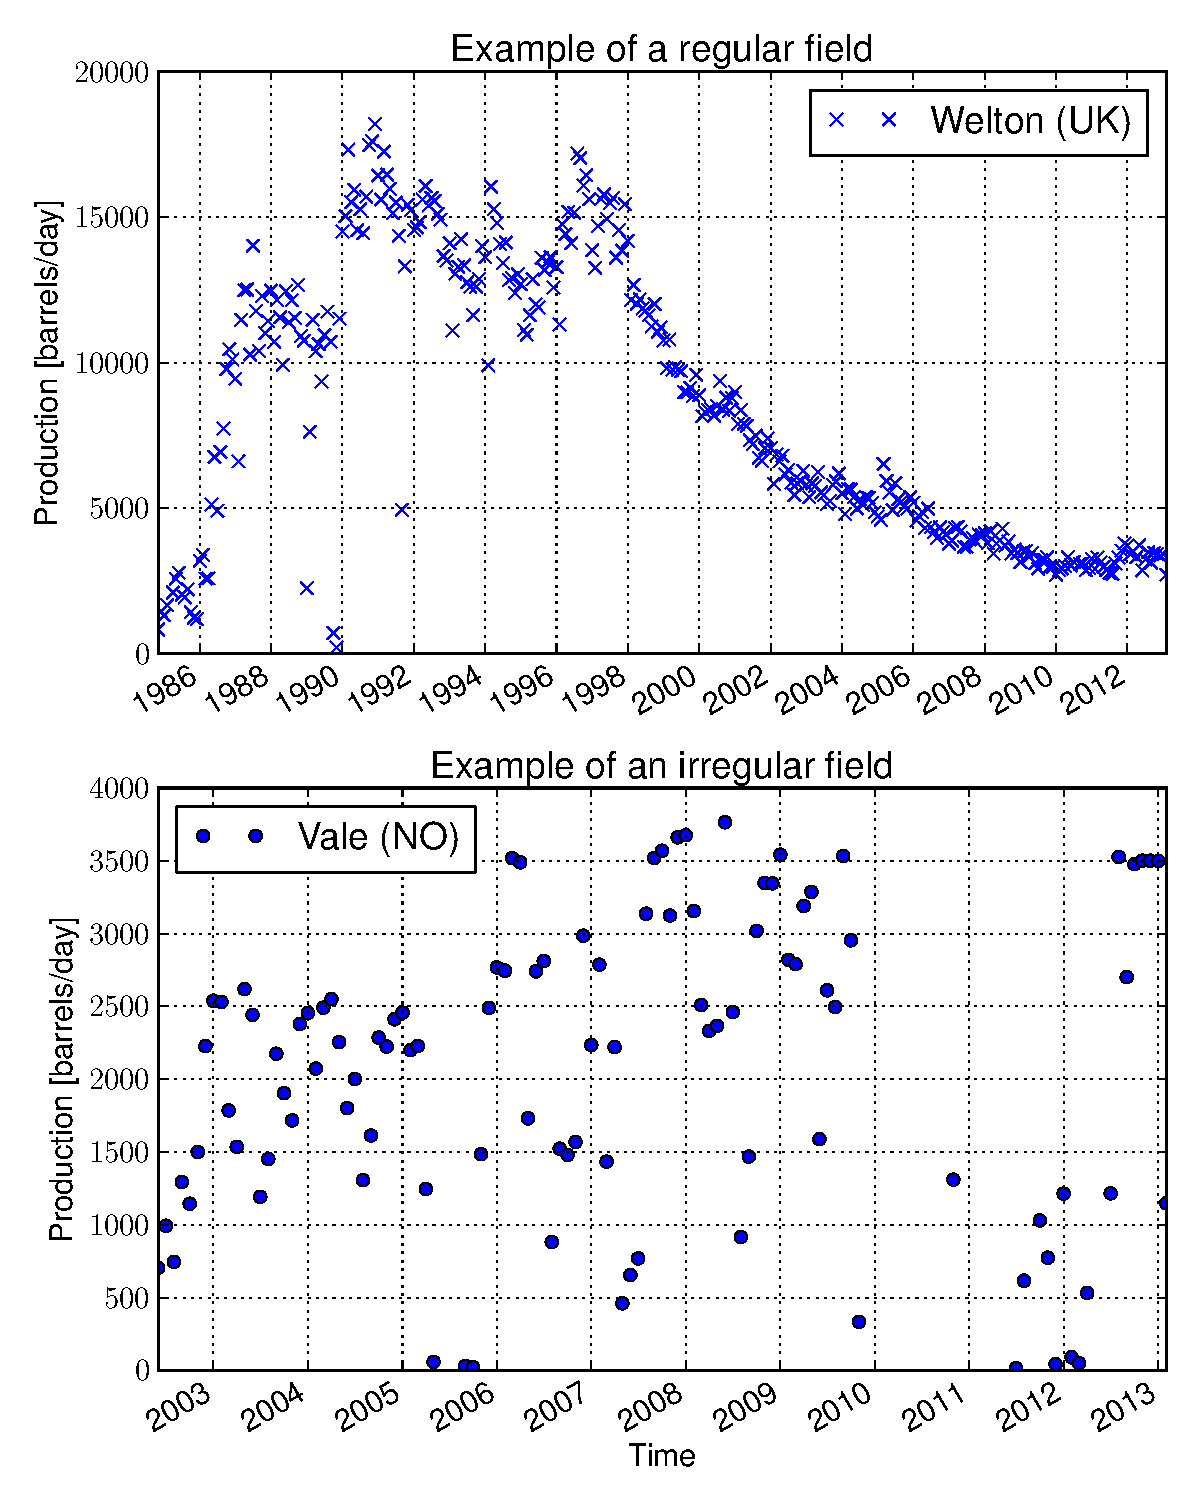
\includegraphics[width=0.5\textwidth]{regular_and_irregular.pdf}
    \caption{Example of a regular and an irregular field.}
    \label{regular_and_irregular}
\end{figure}

\noindent As of January 2013, regular fields make up 85\%, 87\% and z\% of the number of fields and 94\%, 71\% and z'\% of the total oil volume in the Norway, the U.K. and the U.S. respectively. As such, being able to model them is crucial. As can be seen on figure \ref{stretched_exponential}, the stretched exponential (equation \ref{stretched_exponential}) is a good functional form to fit the decay process of regular fields.

\begin{equation} \label{stretched_exponential}
P(t) = P_0 e^{\left (\frac{t}{\tau} \right)^\beta}
\end{equation}

For the minority of irregular fields, we simply modeled their decay as follows. We picked $\tau$ to be the average $\tau$ over the regular fields. We then fixed $\beta$ so that the sum of the fields' production over its lifetime be equal to the official ultimate recovery estimates, when such an estimate is available. %More details can be found in the supplementary materials.

\begin{figure}[H]
    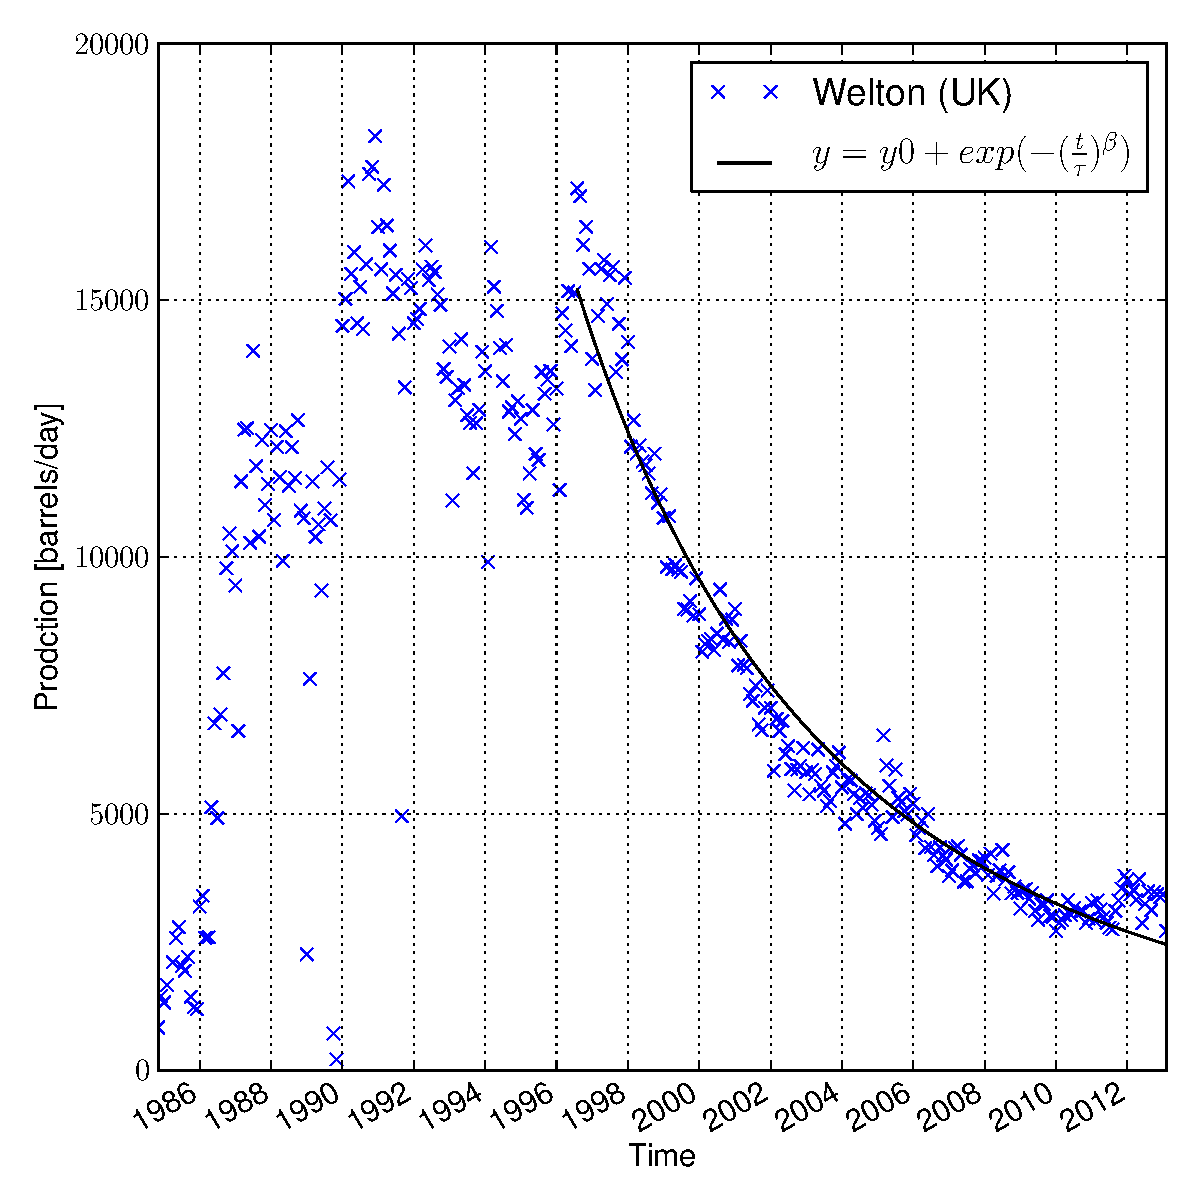
\includegraphics[width=0.5\textwidth]{stretched_exponential.pdf}
    \caption{Stretched exponential fit to the production of Welton. This functional form fits the data well.}
    \label{stretched_exponential}
\end{figure}

\subsection{Discovery rate of new fields}
Knowing the future production rate of existing fields is not enough; new fields will be discovered in the future. The model describing the discovery rate of new fields should satisfy two fundamental observations. 

\begin{enumerate}
\item The rate of new discoveries should tend to zero as time goes to infinity. This is a consequence of the finiteness of the number of oil fields. 
\item The rate of new discoveries should depend on the size of the oil fields. As of today, giant oil fields are discovered much less frequently than dwarfs.
\end{enumerate}

A natural choice for such a model is a non-homogenous poisson process. The Poisson process is a process that generates independent events at  a rate $\lambda$. It is inhomogeneous if the rate is time-dependent, $\lambda \rightarrow \lambda(t)$. The standard way to measure $\lambda(t)$ is to find a functional form for $N(t)$, the number of events (discoveries) up to time $t$. Then, $\lambda(t)$ is simply $\frac{dN(t)}{dt}$. Figure \ref{rate_of_discovery} shows $N(t)$ for Norwegian fields classified according to their size.The logistic curve is a good fit to the data (integral form of equation \ref{logistic}). This implies that after an initial increase, the rate of new discoveries reaches a peak followed by a decrease until no more oil fields are to be found, consistent with our fundamental observations. The results are qualitatively similar for the U.K. and the U.S.

\begin{figure}[H]
    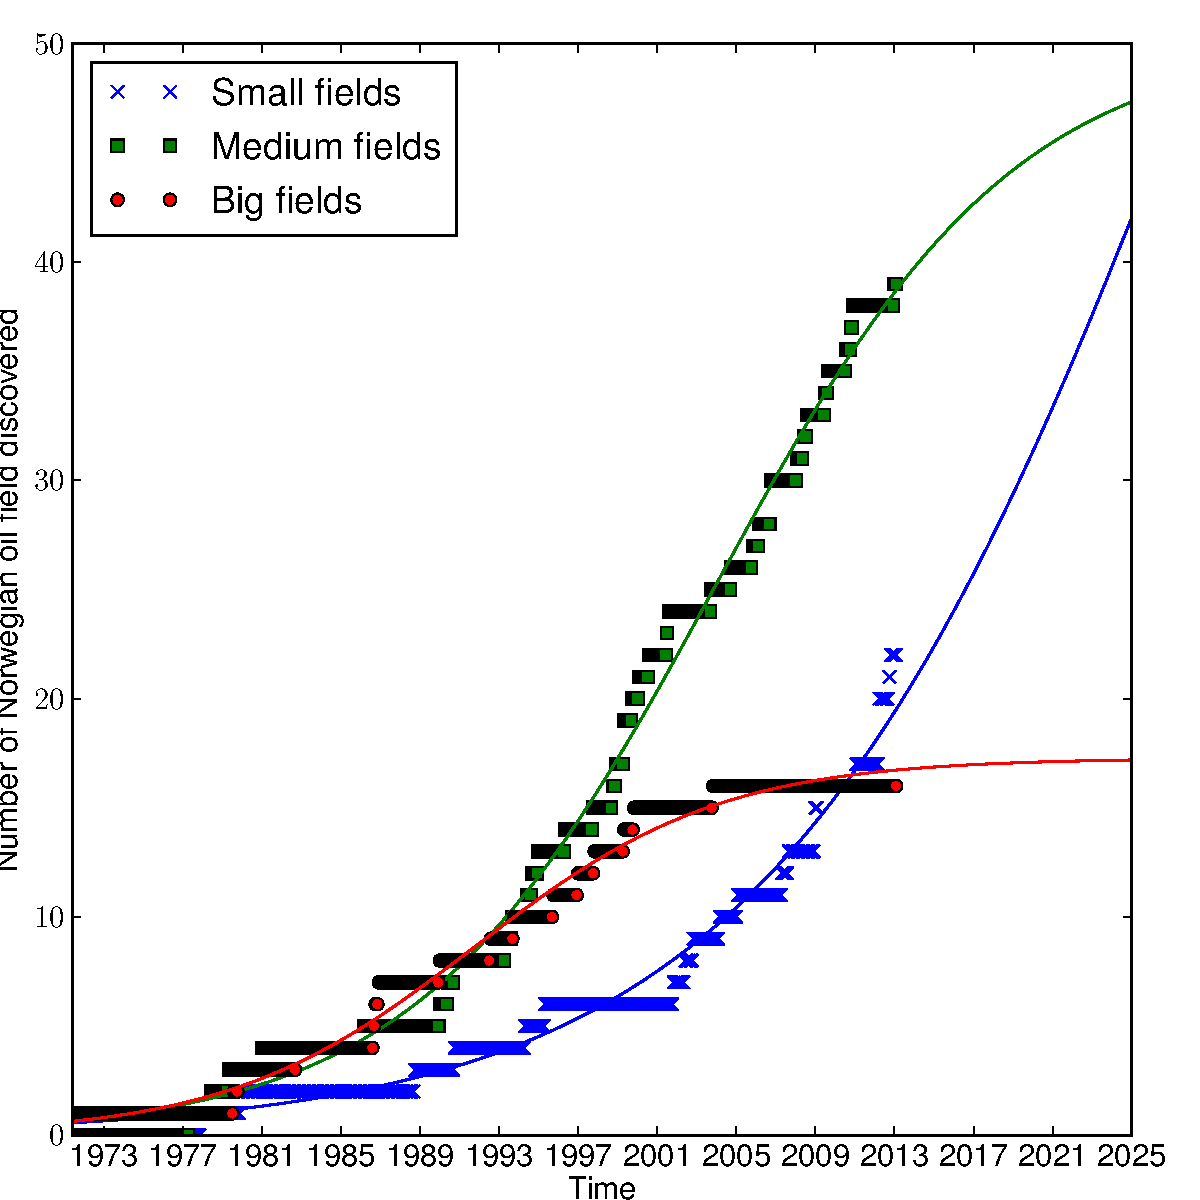
\includegraphics[width=0.5\textwidth]{rate_of_discoveries.pdf}
    \caption{Logistic fit to the number of discoveries for Norway. The discovery rate of new oil fields is dependent on their size. The logistic model suggests that the majority of small oil  fields have not yet been discovered, while the rate of discovery of medium oil fields is in its decreasing phase. Big oil fields are not expected to be discovered anymore. }
    \label{rate_of_discovery}
\end{figure}


%------------------------------------------------

\section{Results}

Simulating future oil production was straightforward. For each country, new oil fields were generated according to the poisson process, with $\lambda(t)$ chosen according to their size. For each of the generated oil fields, its production profile was chosen randomly from one of existing fields within the same size category. Figure \ref{no_uk_2013} shows the average of 1000 (50 on these plots) simulations. For each country, we can immediately notice the non-symmetric shape of the production's dynamics contrary to what Hubbert would have predicted.

\begin{table}[H]
\caption{Remaining oil reserves}
\centering
\begin{tabular}{lllr}
%\toprule
%\multicolumn{2}{c}{Name} \\
%\cmidrule(r){1-2}
Country & Hubbert & our model & $\Delta$ \\
\midrule
Norway & $81 \cdot 10^6$ & $270 \cdot 10^6$ & $-70\%$\\
U.K. & $275 \cdot 10^6$ & $959 \cdot 10^6$ & $-71\%$ \\
U.S.A. & $x$ & $y$ & $z\%$ \\
\bottomrule
\end{tabular}
\end{table}

\begin{figure}[H]
    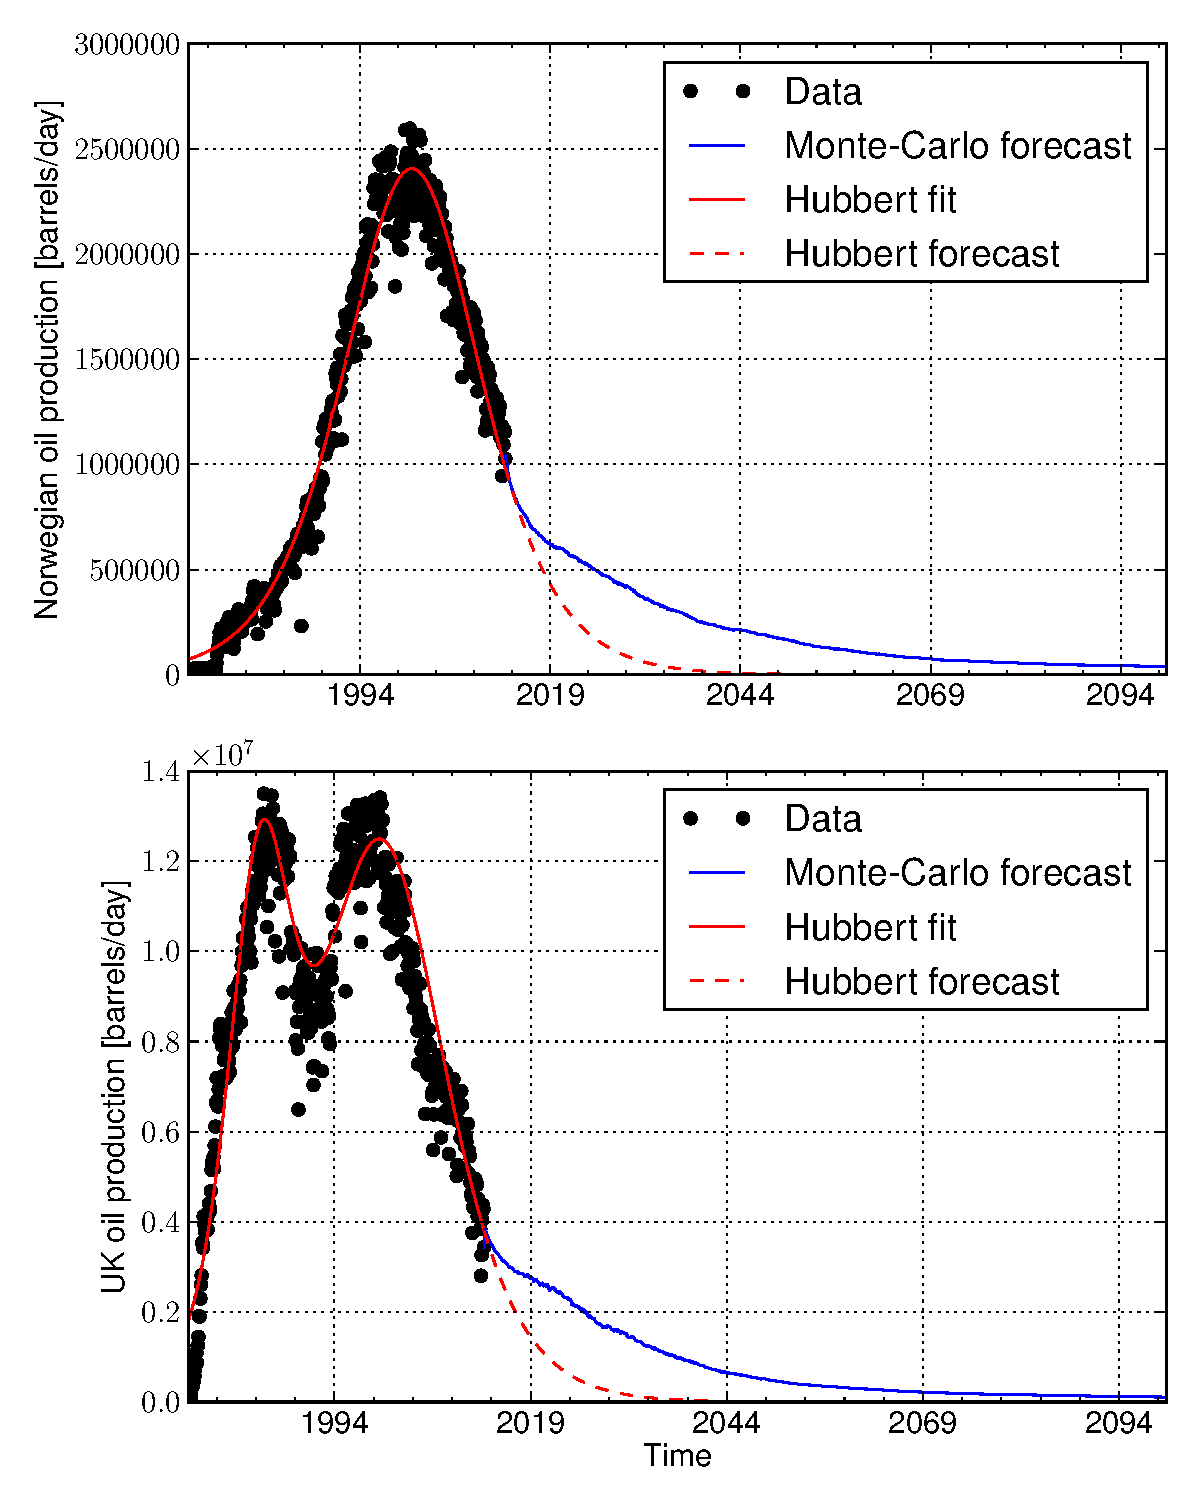
\includegraphics[width=0.5\textwidth]{no_and_uk_2013.pdf}
    \caption{Monte-Carlo and Hubbert forecast based on past production data for Norway (top) and the U.K. (bottom).  In both cases, our model forecasts a significantly slower decay than the Hubbert model.}
    \label{no_uk_2013}
\end{figure}

The difference between our and the Hubbert-based forecast is striking. In the case, of Norway, the standard Hubbert model was used to fit the production data. According to it, Norway's future oil production would decay much faster than in the Monte-Carlo case. As such, the estimated remaining reserves are less than one third of the forecasted value of the Monte-Carlo methodology. In the U.K., oil production faced a change of regime during the early nineties due to technological innovation, giving rise to the inverted "w shape" of the oil production profile. The standard procedure to model oil production in those cases is to use a multi-cyclic Hubbert curve. The multi-cyclic Hubbert model is a generalization of the standard one. Conceptually, it is just a superposition of several standard (single-cyclic) Hubbert curves. Two cycles are commonly used to fit the UK's oil production. The difference between the Hubbert-based methodology and the Monte-Carlo one is very similar to the Norwegian case. The former underestimates the remaining oil reserves by about $70\%$ compared to the latter.\\
Which of the two models is more thrust worthy? Clearly, the implications in adopting one methodology over the other are significant. The only way to answer this question is to backtest them. In other words we ask: "What would have each of the models predicted had we used them 10, 15, 20 years in the past?"


%\begin{table}[H]
%\caption{Example table}
%\centering
%\begin{tabular}{llr}
%\toprule
%\multicolumn{2}{c}{Name} \\
%\cmidrule(r){1-2}
%First name & Last Name & Grade \\
%\midrule
%John & Doe & $7.5$ \\
%Richard & Miles & $2$ \\
%\bottomrule
%\end{tabular}
%\end{table}

%------------------------------------------------

\section{Validation}

For each of the three countries, namely Norway, the U.K. and the U.S.A., we went back in time 10, 15 and 20 years respectively. The reason for chosing an earlier starting point for our backtest in the case of the U.S.A. compared to say, Norway has to do with the number of oil fields available at the time of the backtest. The U.S.A. having the biggest number of oil fields, we could chose an earlier starting point without compromising the quality of our results. Figure \ref{bt} shows the outcome of those tests. In the case of Norway, the production data was taken into account until 2003. Comparing the forecast of both models with the oil production of the subsequent 10 years, we find the predictive power of the Hubbert model is impressive. It perfectlty captures the Norwegian oil production's dynamic between 2003 and 2013. The Monte-Carlo method does not perform as well. After underestimating the Norwegian oil production between 2003 and 2009, it overestimates it between 2009 and 2013. For the U.K. the backtesting was performed on data until 1998. The conclusion is not as obvious as for the previous case. None of the two methods captures perfectly the oil production between 1998 and 2013. The following table summarizes the difference between the two models.

\begin{table}[H]
\caption{Remaining oil reserves}
\centering
\begin{tabular}{llllr}
%\toprule
%\multicolumn{2}{c}{Name} \\
%\cmidrule(r){1-2}
Start & Country & Hubbert & our model & $\Delta$ \\
\midrule
2003 & Norway & $66 \cdot 10^6$ & $251 \cdot 10^6$ & $-74\%$\\
1998 & U.K. & $91 \cdot 10^6$ & $2.1 \cdot 10^9$ & $-43\%$ \\
1993 & U.S.A. & $x'$ & $y'$ & $z'\%$ \\
\bottomrule
\end{tabular}
\end{table}

\begin{figure}[H]
    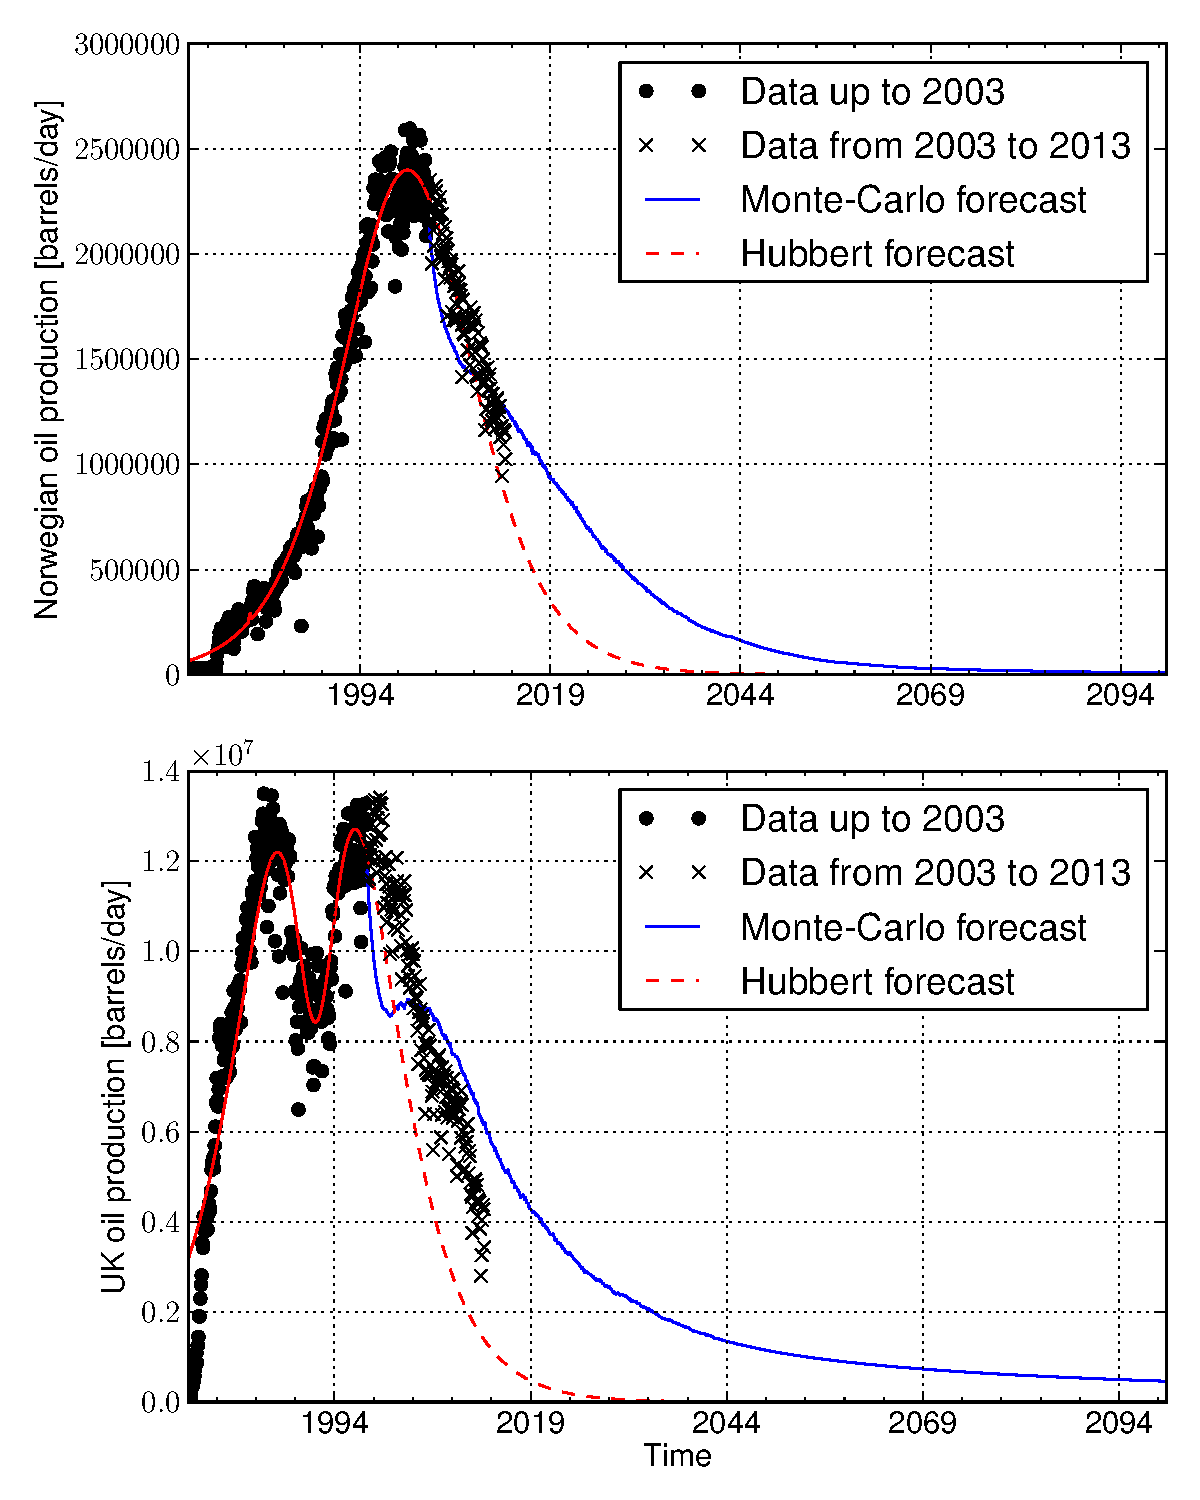
\includegraphics[width=0.5\textwidth]{no_and_uk_bt.pdf}
    \caption{Monte-Carlo and Hubbert forecast based on past production data up to 2003 for Norway (top) and up to 1998 for the U.K. (bottom).  The results can be compared with the subsequent oil production (crosses). In both cases, the Hubbert forecast is more accurate.}
    \label{bt}
\end{figure}

%------------------------------------------------

\section{Conclusion}
We have presented a Monte-Carlo based methodology to forecast future oil production. By extending the oil production of current fields into the future and modeling the discovery rate of new fields, we were able to give forecasts on the future oil production of Norway, the U.K. and the U.S. These forecasts offer significantly scenarios from the ones obtained with standard Hubbert-based methodologies. Indeed, our model gives a 3 times superior estimation of the remaining oil reserves than the standard one. However, our backtesting results seriously questions the credibility of that forecast, since the Hubbert-model clearly outperforms the Monte-Carlo simulation. 
%----------------------------------------------------------------------------------------
%	REFERENCE LIST
%----------------------------------------------------------------------------------------

%\begin{thebibliography}{99} % Bibliography - this is intentionally simple in this template

%\bibitem[Figueredo and Wolf, 2009]{Figueredo:2009dg}
%Figueredo, A.~J. and Wolf, P. S.~A. (2009).
%\newblock Assortative pairing and life history strategy - a cross-cultural
 %study.
%\newblock {\em Human Nature}, 20:317--330.
 
%\end{thebibliography}

%----------------------------------------------------------------------------------------

\end{multicols}

\end{document}
